\documentclass{exam}

\usepackage[utf8]{inputenc}
\usepackage[italian]{babel}
\usepackage[margin=1in]{geometry}
\usepackage{amsmath,amssymb}
\usepackage{tabularray}
\usepackage{array}
\usepackage{multirow}
\usepackage{graphicx}
\usepackage{eurosym}
\usepackage{pgfplots} 
\usepackage{multicol}
\usepackage{geometry}
\usepackage{arev}
\usepackage{siunitx}
\usepackage{hyperref}
\usepackage[
 font=normal % or small or scriptsize
 ]{subfig}
\usetikzlibrary{shapes.geometric}

\linespread{2}
\setlength\answerlinelength{7cm}

% LAYOUT FOGLIO
\geometry{a4paper, top=1cm, bottom=1cm, left=1cm, right=1cm}
\renewcommand{\arraystretch}{1.3}
\setlength{\tabcolsep}{10pt}

\begin{document}
%\input{files_struct/intestazione.tex}  \unskip 

\noindent Classe:\\
Nome e Cognome:


\noindent \rule{\textwidth}{0.4pt}
\Large{Parte 2}\\
\normalsize
Nel seguente grafico vengono riportati i dati dei logaritmi delle frequenze in funzione del rango di ogni parola tipo presente nell'archivio dei contenuti di Wikipedia messo a disposizione sulla piattaforma
\href{https://huggingface.co/datasets/Salesforce/wikitext}{Hugging Face} (Merity et al., 2016) e rielaborato nella prima parte dell'esercitazione.

\begin{figure}[h] 
    \centering 
    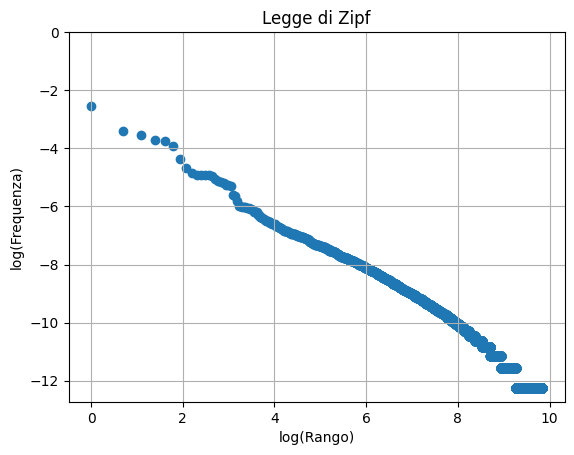
\includegraphics[width=0.5\textwidth]{Legge_Zipf_test}
\end{figure}


\begin{questions}

\question 
Traccia il grafico della retta che meglio interpola i punti e, aiutandoti con un righello, determina il valore del coefficiente angolare $m$ e della quota $q$.

$m=$ \makebox[2cm]{\dotfill}\\[0.3cm]
$q=$ \makebox[2cm]{\dotfill}\\

\question
Scrivi l'equazione della retta.\\[0.3cm]
y= \makebox[0.2\textwidth]{\dotfill}

\question
Sostituisci $y$ con $\log{f}$ e $x$ con $\log{r}$\\[0.3cm]
\makebox[0.3\textwidth]{\dotfill}

\question Svolgi i seguenti passaggi per tovare la legge nascosta tra i dati.

\begin{enumerate}
    \item Applica la proprietà $b\log{a}=\log{a^b}$:
    \[ \log(f) = \log(r^{\dots}) + \dots \]

    \item Applica la funzione inversa del logaritmo (base 10) a entrambi i membri:
    \[ f = 10^{\dots\ldots + \dots} \]

    \item Separa i termini usando le proprietà delle potenze:
    \[ f = 10^{\ldots\ldots} \cdot 10^{\dots} \]

    \item Ottieni la Legge di Zipf:
    \[ f = \dfrac{10^{\dots}}{ r^{\dots}}\]
\end{enumerate}

E' quindi una legge di potenza. Rispondi alle seguenti domande.

\question Cosa succede all'aumentare del rango? Le frequenze aumentano o dinimuiscono? 

\makeemptybox{4cm}


\end{questions}
\end{document}
